\chapter{Gestion des Données et Stratégie de Stockage}
\label{chap:donnees}

\section{Modélisation Relationnelle de la Base de Données}

La persistance des métadonnées et la structuration des sessions de recherche reposent sur un modèle relationnel strict conçu sous \textbf{SQLAlchemy 2.0}. Le modèle relationnel de Perceptra assure une intégrité référentielle absolue, renforcée par des contraintes d'unicité et des suppressions en cascade (\texttt{CASCADE ON DELETE}).

\begin{figure}[htbp]
\centering
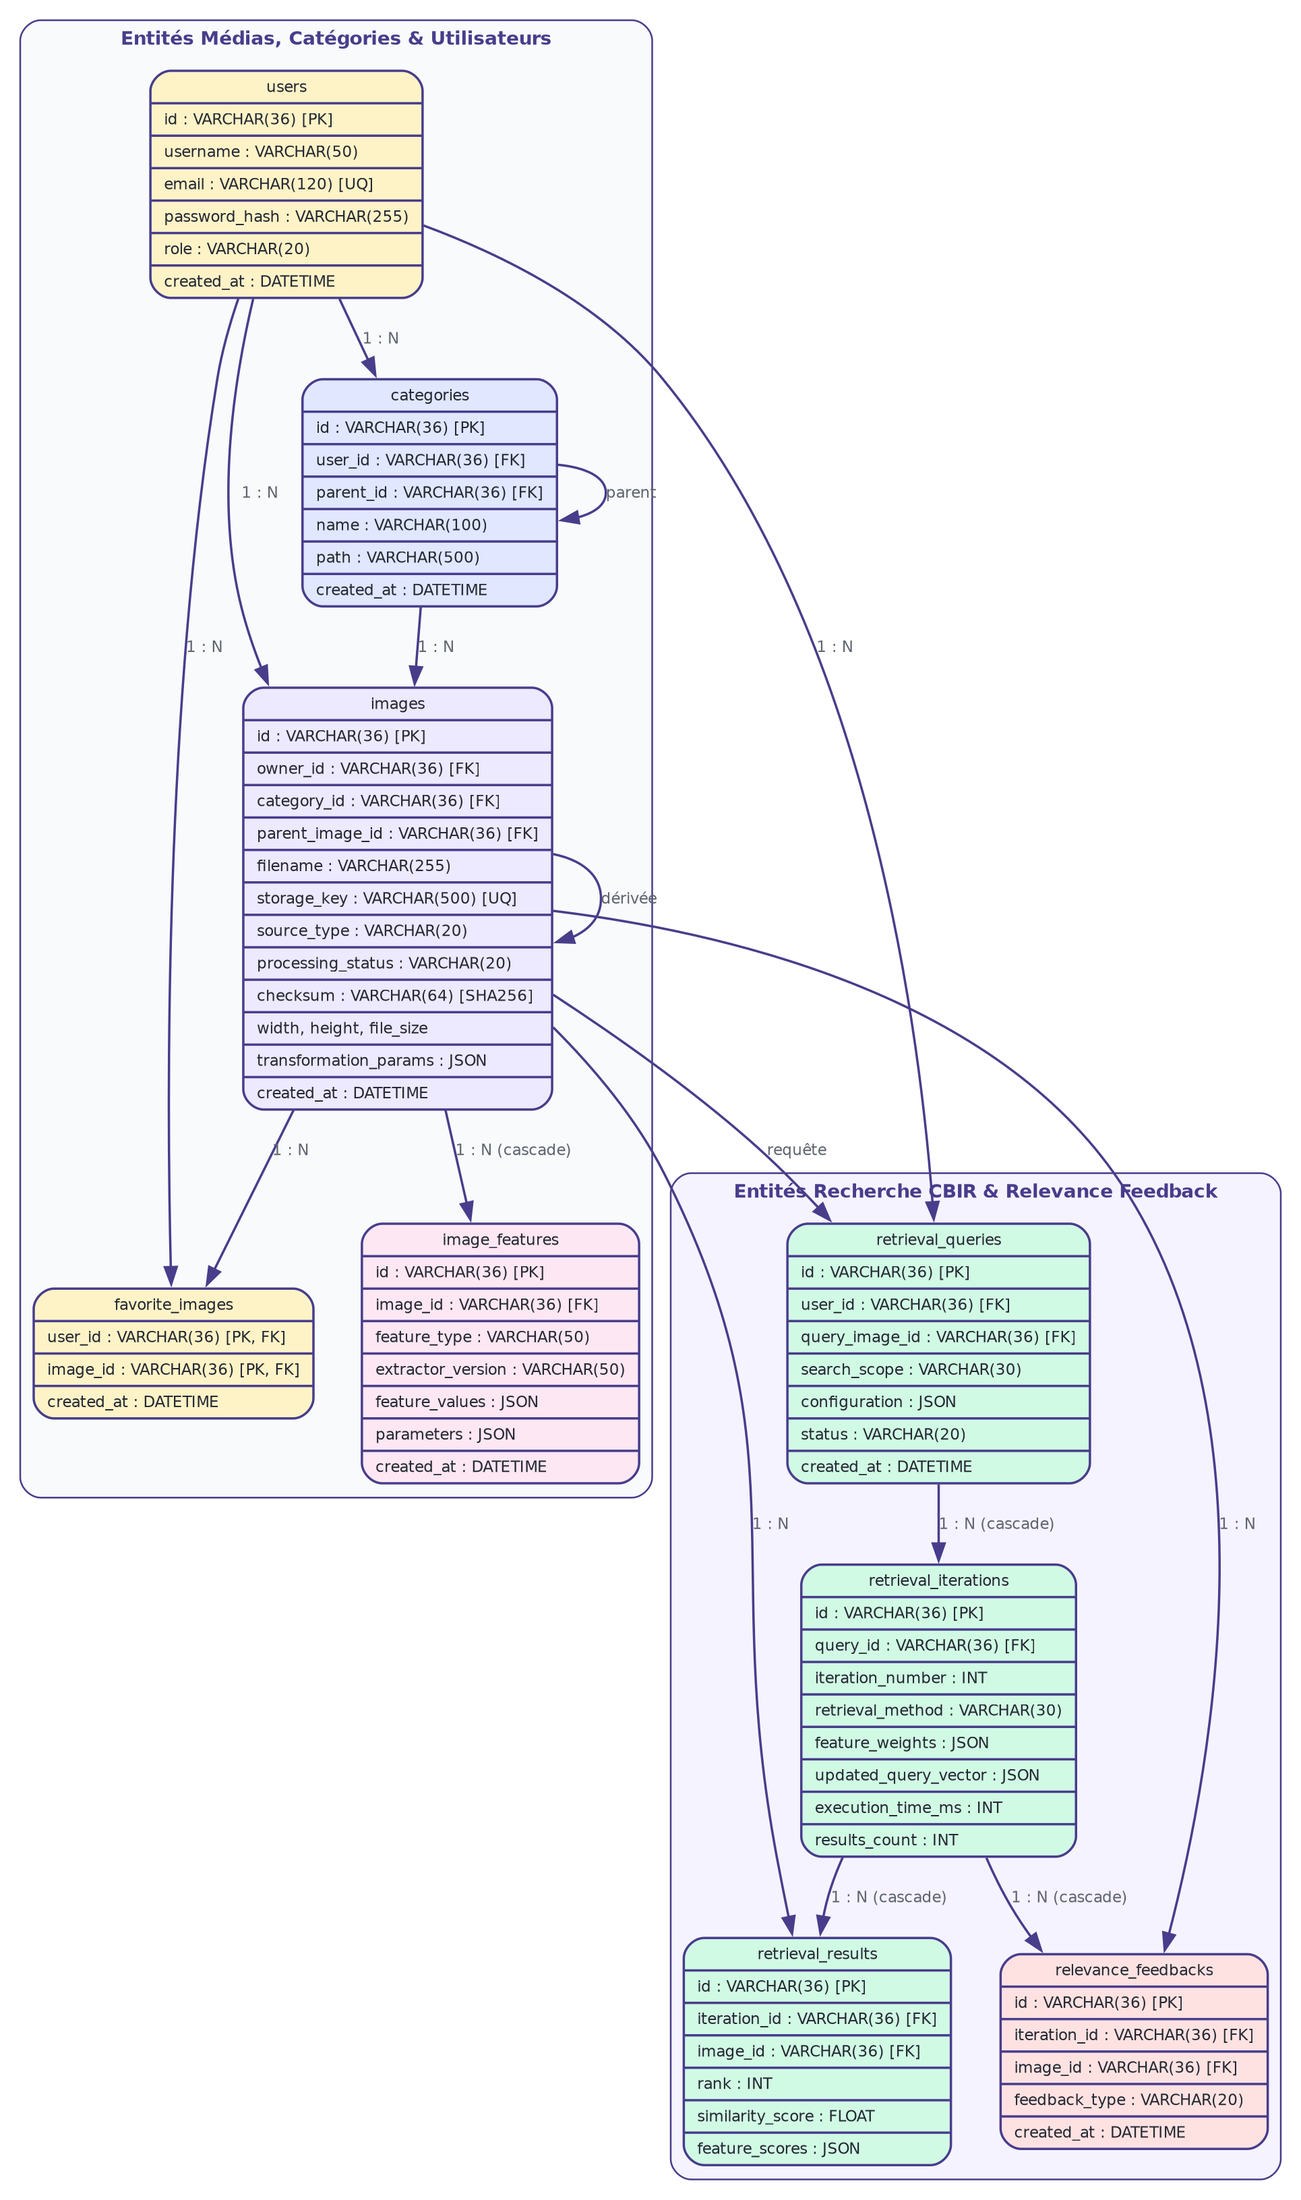
\includegraphics[width=0.48\textwidth]{images/09-schema-relationnel-db.png}
\caption{Schéma Entité-Association complet de la base de données de Perceptra}
\label{fig:schema_db}
\end{figure}

Le tableau~\ref{tab:entites_db} synthétise le rôle et les contraintes des entités principales du schéma.

\begin{table}[H]
\centering
\rowcolors{2}{LightGray}{white}
\begin{tabularx}{\textwidth}{>{\bfseries}p{3.2cm}p{3.0cm}X}
\toprule
\rowcolor{TableHeader}
\color{white}Table & \color{white}Clé Primaire & \color{white}Rôle et Contraintes Notables \\
\midrule
\texttt{users} & \texttt{id (UUID-36)} & Comptes utilisateurs, mot de passe haché par PBKDF2-HMAC-SHA256, rôle (\texttt{admin}, \texttt{user}). \\
\texttt{categories} & \texttt{id (UUID-36)} & Organisation arborescente, clé étrangère réflexive \texttt{parent\_id} pour la hiérarchie parent-enfant, chemin calculé \texttt{path}. \\
\texttt{images} & \texttt{id (UUID-36)} & Métadonnées physiques, clé de stockage unique \texttt{storage\_key}, condensat \texttt{checksum} (SHA-256 indexé), dimensions, source (\texttt{dataset}, \texttt{upload}, \texttt{derived}). \\
\texttt{image\_features} & \texttt{id (UUID-36)} & Vecteurs de descripteurs JSON. Contrainte d'unicité stricte \texttt{uq\_image\_feature\_type\_version} sur \texttt{(image\_id, feature\_type, extractor\_version)}. \\
\texttt{retrieval\_queries} & \texttt{id (UUID-36)} & Sessions de recherche initialisées par l'utilisateur, traçabilité du périmètre (\texttt{search\_scope}) et statut. \\
\texttt{retrieval\_iterations} & \texttt{id (UUID-36)} & Itérations successives au sein d'une session, numéro ordonné, méthode de recherche (\texttt{initial}, \texttt{fre}), poids de caractéristiques appliqués, temps en ms. \\
\texttt{retrieval\_results} & \texttt{id (UUID-36)} & Classement des $K$ résultats par itération, rang d'ordonnancement, score global et décomposition par descripteur. \\
\texttt{relevance\_feedbacks} & \texttt{id (UUID-36)} & Annotations interactives de l'utilisateur sur une itération donnée (\texttt{relevant}, \texttt{irrelevant}), horodatées. \\
\bottomrule
\end{tabularx}
\caption{Spécification fonctionnelle des entités de la base de données}
\label{tab:entites_db}
\end{table}

\section{Stratégie de Stockage Hybride et Intégrité Binaire}

Perceptra refuse le stockage direct des flux binaires dans la base de données (colonnes \textit{BLOB}), qui dégrade les tampons mémoire. Le système met en œuvre une \textbf{architecture de stockage hybride}~:
\begin{enumerate}
    \item \textbf{Plan de Données (Système de Fichiers)~:} Les fichiers images bruts sont enregistrés directement sur le volume physique sous des clés UUID4 horodatées (\texttt{storage/uploads/YYYY/MM/<uuid>.<ext>}).
    \item \textbf{Plan de Contrôle (Base SQL)~:} La base de données ne stocke que le descripteur d'accès logique (\texttt{storage\_key}), l'empreinte cryptographique SHA-256, les dimensions et les signatures vectorielles.
    \item \textbf{Vérification d'Intégrité SHA-256~:} Chaque téléversement donne lieu au calcul de son condensat SHA-256. L'index de la colonne \texttt{checksum} détecte instantanément les doublons stricts, économisant l'espace disque et le temps de calcul.
\end{enumerate}

\section{Ingestion du Dataset GHIM-10K et Migrations}

Le jeu de données de référence \textbf{GHIM-10K}~\cite{kaggle_ghim10k} rassemble \textbf{10\,000 images} photographiques réparties en 20 classes thématiques de 500 images chacune (avions, navires, automobiles, feux d'artifice, fleurs, chevaux, montagnes, etc.).

Le service \texttt{DatasetService} (\texttt{src/services/dataset\_service.py}) ingère et pré-indexe cette volumétrie par blocs transactionnels de 500 enregistrements (\texttt{db.session.bulk\_save\_objects}). L'opération s'exécute en environ 18 minutes sur un processeur multi-c\oe{}urs standard, pour un volume de base de données final inférieur à 65 mégaoctets. Les modifications de schéma sont rigoureusement versionnées et appliquées via \textbf{Flask-Migrate} / Alembic.
